\documentclass{article}
\usepackage{amsmath}
\usepackage{hyperref}
\usepackage{amsfonts}
\usepackage{bookmark}
\usepackage{float} 
\usepackage{graphicx}
\usepackage{makeidx}
\usepackage{pgfplots}
\usepackage[letterpaper, total={7.5in, 10in}]{geometry}


\makeindex
\pgfplotsset{compat=1.18}
\newcommand{\CURL}{\operatorname{curl}}
\newcommand{\DIV}{\operatorname{div}}
\begin{document}
\title{Proving Shell Theorem the Shell}
\author{Elias Xu}
\date{\today}
\maketitle

\setlength{\parindent}{0pt}


\section{Intro}

Just setting out to prove the shell theorem inside the shell.

\begin{figure}[H]
    \centering
    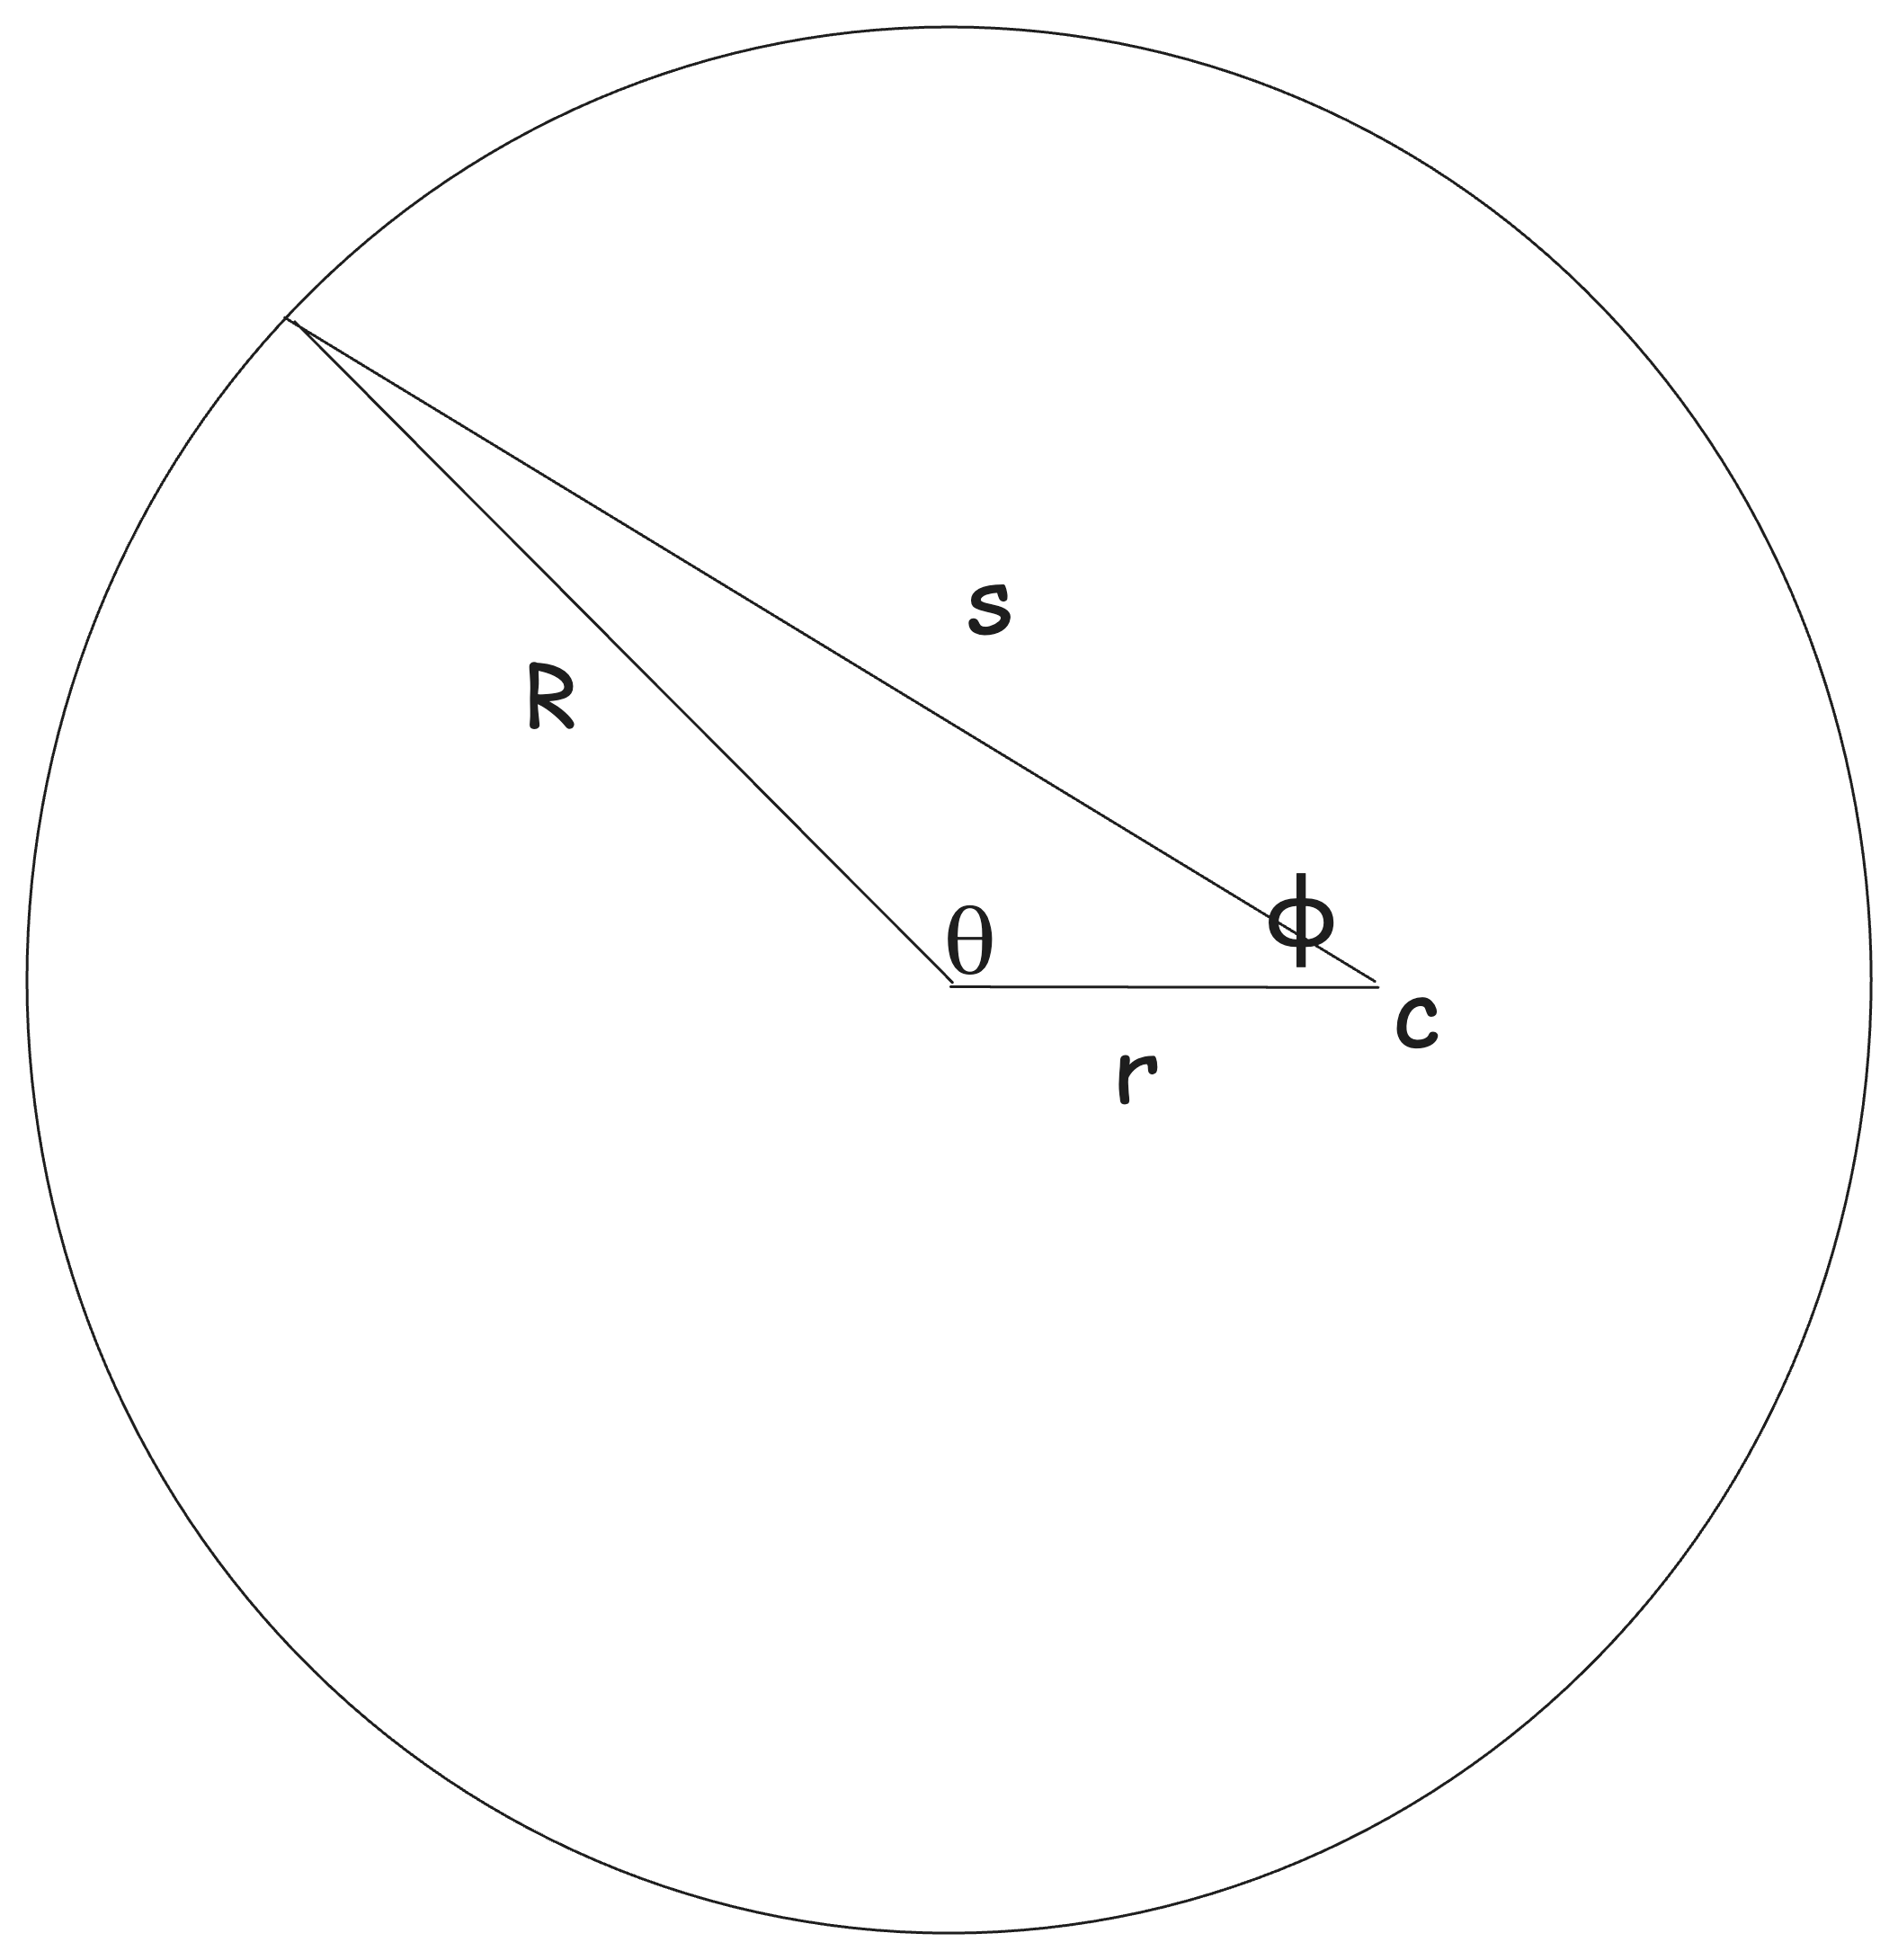
\includegraphics[width=0.5\textwidth]{figures/init_shape.png}
    \caption{Reference}
\end{figure}

We first start with the formula for gravity.

$$F = \frac{G m M }{r^2}$$

We then have to represent it for a single point on the sphere. The cosine because we have to remember stuff cancels out.

$$\delta F = \frac{G m \delta M}{s^2} \cos(\phi)$$

Then we have to convert the terms and the integrand. 

$$\delta M = \sigma \delta A$$
$$ = \sigma R \sin(\theta) \delta s = \sigma 2 \pi R^2 \sin(\theta ) \delta \theta$$
$$\delta F = \frac{G m 2 \pi R^2 \sigma  \sin(\theta) \delta \theta}{s^2}$$

We then need to do additional conversions given the number of terms that we are dealing with here. Let's rewrite some different variables. 

$$R^2 = s^2 \sin^2 \phi + (s\cos\phi - r)^2 = s^2 + r^2 - 2sr\cos\phi$$
$$cos \phi = \frac{- R^2 + s^2 + r^2}{2sr}$$

Also convert $\delta s$ and $\delta \theta$, the negative cos is because the theta is the wrong side

$$s^2 = R^2\sin^2\theta + (r - R\cos\theta)^2 = R^2 + r^2 - 2rR\cos\theta$$
$$2s\delta s = 2rR \sin \theta \delta \theta $$
$$\delta \theta = \frac{s \delta s}{rRsin\theta}$$

Substituting all the Substitutions:

$$\delta F = \frac{G m 2 \pi R^2 \sigma  \sin(\theta) }{s^2}\left(\frac{s \delta s}{rRsin\theta}\right) \left(\frac{-R^2 + s^2 + r^2}{2sr}\right)$$
$$\delta F = \frac{G m M}{4 \pi R r^2} \left(\frac{- R^2 + s^2 + r^2}{s^2}\right) = \frac{G m M}{4 \pi R r^2} \left( 1 + \frac{ r^2 - R^2}{s^2}\right) $$
$$F = \frac{G m M}{4 \pi R r^2} \int_{R-r}^{R+r} 1 + \frac{r^2 - R^2}{s^2} \delta s = 0$$

\section{Gravastar}


\begin{figure}[H]
    \centering
    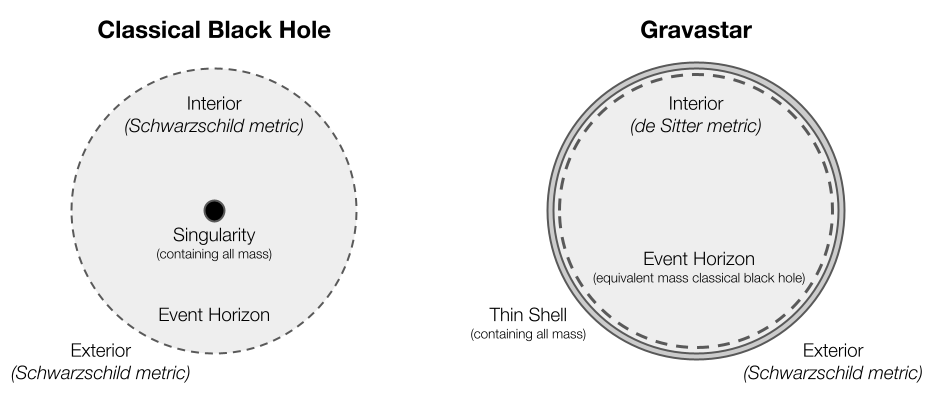
\includegraphics[width=0.5\textwidth]{figures/Gravastar.png}
    \caption{Reference}
\end{figure}

\begin{enumerate}
    \item Alternative to Black holes
    \item Massive Starts -> supernova -> either black hole or neutron start 
    \item Gravastar -> when it collapses, creates energy from core which pushes out and which fights collapsing rest of the star, creating new matter ultrathin bubble
    \item Empty but full of energy vacuum , 1e44 more energy than a black hole
    \item Give idea of big bang, because u get new dimensions with this
    \item We get stuff from 2 collapsing gravastars / black holes
\end{enumerate}


\end{document}